\subsection{$\displaystyle \lim_{x\to \infty}\bracket[s]{\sqrt{x^2-x}-x}$}
% \begin{gather}
% \begin{aligned}
%     \sqrt{x^2-x}-x &= \bracket{\sqrt{x^2-x}-x} \cdot \frac{\sqrt{x^2-x}+x}{\sqrt{x^2-x}+x}
%     = \frac{\bracket{\sqrt{x^2-x}-x}\bracket{\sqrt{x^2-x}+x}}{\sqrt{x^2-x}+x}\\
%     &= \frac{\bracket{\sqrt{x^2-x}}^2-x^2}{\sqrt{x^2-x}+x} 
%     = \frac{x^2-x-x^2}{\sqrt{x^2-x}+x} = \frac{-x}{\sqrt{x^2-x}+x}\\
%     &= \frac{-1}{\frac{1}{x}\sqrt{x^2-x}+1} = -\frac{1}{\sqrt{\frac{x^2}{x^2}-\frac{x}{x^2}}+1}
%     = -\frac{1}{\sqrt{1-\frac{1}{x}}+1}  
% \end{aligned}
% \end{gather}
% \begin{gather}
%     \lim_{x\to\infty} \bracket[s]{\sqrt{x^2-x}-x} 
%     = \lim_{x\to\infty} -\frac{1}{\sqrt{1-\frac{1}{x}}+1} \\
%     \mbox{as } x \to \infty\mbox{: } \frac{1}{x} \to  0^+; \quad \sqrt{1-\frac{1}{x}} \to  1^-;
%     \quad \sqrt{1-\frac{1}{x}}+1 \to 2^-\\
%     \result{\lim_{x\to\infty} \bracket[s]{\sqrt{x^2-x}-x} = -\frac{1}{2}^-= -0.5^-}
% \end{gather}



Let $f(x)=\sqrt{x^2-x}-x = \sqrt{x(x-1)}-x = \sqrt{\bracket{x-0.5}^2-0.25}$\\
Then: $D_f = \R\backslash\, ]0;1[\ =\ ]-\infty;0] \cup [1;\infty[$\\
We want: $\displaystyle \lim_{x\to \infty}f(x)$

\begin{gather}
\begin{aligned}
    \lim_{x\to\infty}\bracket[s]{\sqrt{x^2-x}-x} &< \lim_{x\to\infty}\bracket[s]{\sqrt{x^2}-x}
     = \lim_{x\to\infty}\bracket[s]{\abs{x} - x} = 0\\
    \implies \lim_{x\to \infty} f(x) &< 0
\end{aligned}
\end{gather}

\begin{gather}
\begin{aligned}
\lim_{x\to\infty}\bracket[s]{\sqrt{x^2-x}-x} &> \lim_{x\to\infty}\bracket[s]{\sqrt{x^2-2x+1}-x}
 = \lim_{x\to\infty}\bracket[s]{\sqrt{\bracket{x-1}^2}-x} = \lim_{x\to\infty}\bracket[s]{\abs{x-1}- x}\\
    \lim_{x\to\infty}f(x) &> \lim_{x\to\infty}\bracket[s]{ x-1-x } = -1\\
    \implies \lim_{x\to \infty} f(x) &>  -1
\end{aligned}
\end{gather}

\begin{gather}
\implies \lim_{x\to\infty} f(x) \in\ ]-1;0[\\
    \mbox{set } L = \lim_{x\to \infty} f(x)
\end{gather}

For visualizing which quadratic is ``bigger'' and therefore determen the inequalities.\\
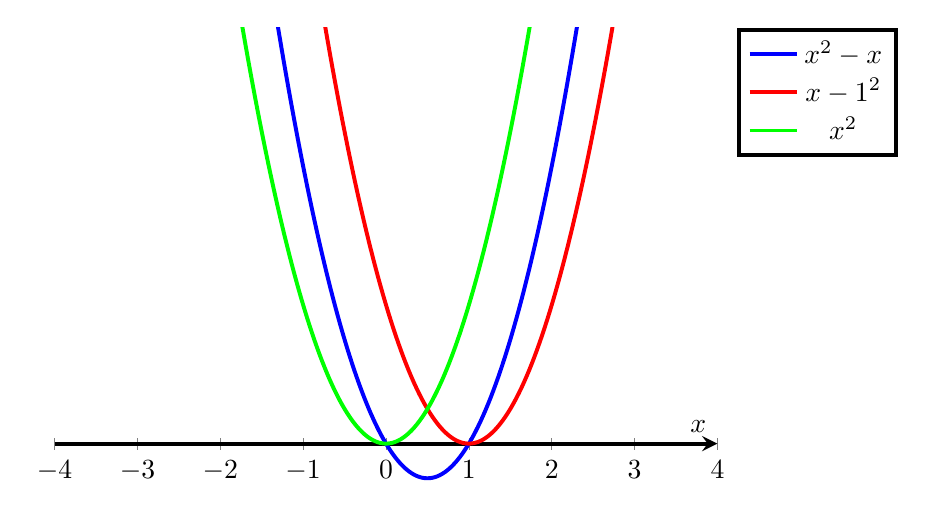
\begin{tikzpicture}
\begin{axis}[
    width=10cm,
    axis lines=center,
    hide obscured x ticks=false, %so that 0 will show up
    hide obscured y ticks=false,
    hide y axis,
    xmin=-4, xmax=4,
    ymin=-1, ymax = 3,
    xlabel={$x$},
    samples=325,
    line width=0.05cm,
    legend pos=outer north east,
]
    \addplot [blue] {(x^2-x)};
    \addlegendentry{$x^2-x$}

    \addplot [red] {(x-1)^2};
    \addlegendentry{$\bracket{x-1}^2$}

    \addplot [green] {x^2};
    \addlegendentry{$x^2$}
\end{axis}
\end{tikzpicture}


Let $h_a(x) = \sqrt{\bracket{x-a}^2}-x$\\
Then as long as $\bracket{x-a}^2$ and $x^2-x$ intersect each other,
the limes of $\displaystyle \lim_{x\to\infty} \bracket[s]{f(x)-h_a(x)}$ will not be finite.
But for $\displaystyle \lim_{x\to\infty}f(x) = \lim_{x\to\infty}h_a(x)$ to be true, the limes must be finite.\\
So we need to find an $a$ such that $\bracket{x-a}^2=x^2-x$ has no solutions:
\begin{gather}
\begin{aligned}
    x^2-x &= \bracket{x-a}^2\\
    x^2-x &= x^2 - 2ax + a^2\\
    2ax-x &= a^2\\
    x(2a-1) &= a^2
\end{aligned}\\
    x = \frac{a^2}{2a-1} = \frac{a^2}{2\bracket{a-\frac{1}{2}}}
\end{gather}
$\implies a=\frac{1}{2}$ because only then
the equation $\bracket{x-a}^2=x^2-x$ has no solutions.
\begin{gather}
\begin{aligned}
    \implies \lim_{x\to\infty}f(x) &= \lim_{x\to\infty}h_{\frac{1}{2}}(x)\\
    &= \lim_{x\to\infty} \bracket[s]{\sqrt{\bracket{x-\frac{1}{2}}^2}-x}\\
    &= \lim_{x\to\infty} \bracket[s]{\abs{x-\frac{1}{2}}-x}\\
    &= \lim_{x\to\infty} \bracket[s]{x-\frac{1}{2}-x} = -\frac{1}{2}\\
\end{aligned}\\
\result{\lim_{x\to\infty}\bracket[s]{\sqrt{x^2-x}-x} = -\frac{1}{2}}
\end{gather}
